\chapter{QUADRO METODOLÓGICO}

	\par Nesse capítulo serão apresentados os métodos adotados para se realizar a
pesquisa, tais como tipo de pesquisa, contexto, procedimentos, entre outros.

\section{Tipo de pesquisa}
	
	\par Uma pesquisa é ato de buscar e procurar pela resposta de algo.
\citeonline[p. 15]{markoni2002} definem pesquisa como “uma indagação minuciosa
ou exame crítico e exaustivo na procura de fatos e princípios”.

	\par Existem diversos tipos de pesquisa, no entanto percebeu-se que para o
propósito desta, a mais indicada foi a pesquisa aplicada, pois foi desenvolvido
um projeto real que poderá ser utilizado por qualquer instituição de ensino,
mas que não mudará a forma com que as pessoas recebam suas informações, apenas
acrescenta mais uma forma de consultá-las.

	\par Segundo \citeonline[p. 15]{markoni2002}, uma pesquisa do tipo aplicada
“Caracteriza-se por seu interesse prático, isto é, que os resultados sejam
aplicados ou utilizados, imediatamente, na solução de problemas que ocorrem na
realidade”.

	\par Dessa maneira, percebeu-se que a pesquisa enquadra-se no tipo de
	pesquisa aplicada, pois resolveria um problema específico, e para isso foi criado uma
aplicativo para dispositivos móveis que facilitará aos graduandos acessarem o
sistema \textit{web} de uma universidade.

\section{Contexto de pesquisa}

	\par Essa pesquisa será benéfica a qualquer instituição educacional que possua
um portal \textit{online}, pois facilitará o acesso dos discentes às suas
informações escolares.

	\par Foi criado um aplicativo para dispositivos móveis, porém inicialmente
apenas para a plataforma \textit{Android}, o qual notifica os usuários quando
há alguma mudança, como por exemplo, ao ser lançada uma nota.
	
	\par O aluno consegue acessar o aplicativo com o mesmo \textit{login} do
sistema \textit{web}. O utilitário acessa o \textit{webservice} que é
responsável por buscar as informações no banco de dados e apresenta-las no
dispositivo móvel.
	
\section{Instrumentos}

	\par Pode-se dizer que um questionário é uma forma de coletar informações
através de algumas perguntas feitas a um público específico. Segundo
\citeonline{gunther2003}, questionário pode ser definido como um conjunto
de perguntas que mede a opinião e interesse do respondente.
	
	\par Foi realizado um questionário simples, que esta apresentado na figura
\ref{fig:exemplo4}, contendo quatro perguntas e enviado para \textit{e-mails} de
alguns alunos da universidade. O foco desse questionário era saber o motivo pelo qual
os usuários mais acessavam o portal do aluno e se tinham alguma dificuldade em
encontrar o que procuravam. Obteve-se um total de treze respostas, no qual
pode-se perceber que a maioria dos entrevistados afirmam terem dificuldades
para encontrar o que precisam e que o sistema não avisa quando ocorre alguma
alteração. Sobre o motivo do acesso cem por cento respondeu que entram no
sistema web para consultar suas notas.

\begin{figure}[h!]
	\centerline{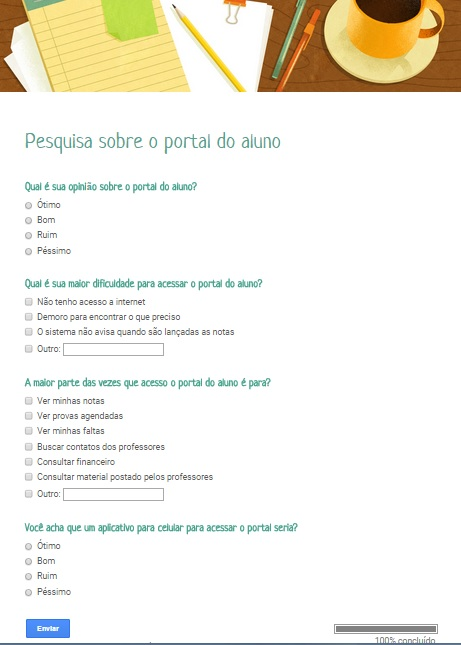
\includegraphics[scale=0.5]{./imagens/imagem4.png}}
	\caption[Quetionário Aplicado]{Quetionário Aplicado.
	 \textbf{Fonte:}Elaborado pelos autores.}
	\label{fig:exemplo4}
\end{figure}

\pagebreak

	\par Outra forma utilizada para realizar a pesquisa foram as reuniões, ou seja,
unir-se com uma ou mais pessoas em um local, físico ou remotamente para tratar
algum assunto específico. Para \citeonline{ferreira1999}, reunião é o ato
de encontro entre algumas pessoas em um determinado local, com finalidade de tratar
qualquer assunto.

	\par Durante a pesquisa, foram realizadas reuniões entre os participantes com o
objetivo de discutir o andamento das tarefas pela qual cada integrante ficou
responsável. Além disso entravam em discussão, nessas reuniões, o cumprimento
das metas propostas por cada participante e o estabelecimento de novas metas.
Foi utilizada nessa pesquisa, referencias em livros, revistas, manuais e web
sites.


\section{Procedimentos}
	
	\subsection{Uml}
	
			\par O primeiro procedimento realizado para chegar ao resultado final 
		da pesquisa proposta, foi delinear a arquitetura do \textit{software} através
		da linguagem UML, fazendo uso de alguns diagramas oferecido pela mesma, como
		ferramenta de apoio. A contrução desses diagramas só foi possível com a
		instalação da ferramenta Astah.
			
			\par Para o aplicativo \textit{Android}, fez-se necessários os diagramas de
		classe, de caso de uso principal e de atividade.
		
			\par Para a contrução do \textit{software} proposto por essa pesquisa além do
		levantamento de requisitos que é peculiar da contrução de qualquer
		\textit{software}, foram também utilizados alguns diagramas da UML. Entre os
		diagramas usado estão:
			\begin{itemize}
			  
			  \item Diagrama de casos de uso;
			  
			  \item Diagrama de sequência;
			  
			  \item Diagrama de Entidade e Relacionamento (ou Modelo de Entidade e
			  Relacionamento )
			
			\end{itemize}
	
	
	\subsection{Resto}
	
		\par Para iniciar o desenvolvimento do aplicativo, primeiramente fez-se
	necessária a instalação e configuração da plataforma \textit{Android Studio} e
	\textit{Android SDK}. Ao concluir essa tarefa, deu-se o início ao aplicativo
	\textit{Android}.

		\par O primeiro passo foi a criação de uma \textit{activity} que é o
	\textit{main}, ou seja a qual executará a aplicação quando for iniciada.
	A \textit{activity} escolhida é denominada \textit{Navigation Drawer Layout}.
	Com ela é possível criar, do lado esquerdo, uma lista que funcionará como um
	menu, com as opções \textit{Home}, Notas, Faltas, Provas Agendadas e Sair.
	Essas opções ficam escondidas e só apareceram quando clicado no canto superior
	esquerdo.

		\par Sempre que a aplicação é iniciada ou quando retorna-se para a
	\textit{Home}, é mostrado ao usuário uma lista de \textit{links} uteis. Para
	que essa lista aparecesse foi utilizada uma \textit{activity} chamada de
	\textit{Master/ Deital Flow} que já traz consigo o \textit{widget} de
	\textit{ListView}. Essa \textit{activity} mostrara as seguintes opções: Univás,
	MEC, FIES, Prouni e Google Acadêmico. Ao clicar em um desses itens será chamada
	uma atividade que mostrará os detalhes do item escolhido, nesse caso na
	\textit{activity} que detalhará o item foi utilizada uma \textit{WebView} que
	mostrará a página web no espaço reservado. Dessa maneira, quando for clicado na
	opção Univas será carregada o site da universidade no aplicativo.

		\par Logo após foram criadas três novas \textit{activities} chamadas de
	\textit{Blank Activity}, as quais listarão as matérias. Nelas foram inseridas o
	\textit{widget ExpandableListView}, para que quando clicado em um item listado,
	ele expande e mostra mais informações, com isso quando se escolhe o menu notas,
	será mostrada uma \textit{activity} que listará todas as matérias cursadas pelo
	aluno e ao clicar em uma delas mostrará as notas dessa disciplina.

		\par Foi criada uma classe chamada BuscaDados, ela tem por finalidade receber
	os dados do \textit{webservice}, salva-los no banco de dados local do
	aplicativo e os entregar para as classes que implementam o \textit{Adapter}
	para listar as informações.

		\par No arquivo \textit{AndroidManifest.xml} foi necessário alterar a opção
	\textit{Android:icon}, que define qual será o ícone do aplicativo, por padrão
	ele apresenta o mascote do \textit{Android}, no entanto foi definida uma imagem
	do logo da universidade. Foi necessário também incluir uma \textit{tag} de
	\textit{users-permission} para \textit{web}, que obriga o usuário a permitir o
	uso da \textit{internet} pelo aplicativo.

		\par O \textit{Android Studio} tem uma facilidade para se trabalhar com
	controladores de versão, nesse caso foi escolhido o \textit{GitHub}. Nele foi
	criado uma pasta e compartilhada entre os participantes e por fim configurado
	no IDE para que cada um possa ter a versão mais atualizada do projeto.
	
		\par No que diz respeito à contrução do \textit{webservice}, foi necessário a
	intalação e configuração de um ambiente de desenvolvimento compatível com as
	necessidades apresentadas pelo \textit{software} e que foram levantadas
	através dos requisitos. Foi instalado o \textit{Servlet Container Apache
	Tomcat} em sua versão de número 7. O \textit{Servlet Container} foi instalado
	para que o \textit{Web Service} pudesse fornecer os serviços necessários para
	o consumo de dados do Aplicativo \textit{Android}, haja vista que
	\textit{Apache tomcat} faz uso amplo do protocolo HTTP\footnote{HTTP -
	Hypertext Transfer Protocol} e da plataforma \textit{Java} de desenvolvimento.
			
		\par Para armazenar os dados gerados e/ou recebidos foi necessário fazer a
	intalação do Sistema Gerenciador de Banco de Dados(SGBD) \textit{PostGreSql} na
	sua versão de número 9.2. Através de um levantamento de requisitos parciais e das
	reuniões entre os participantes foi possível construir um Diagrama de Entidade
	e Relacionamento, no qual ficou definido a estrutura do banco de dados da
	aplicação. A figura \ref{fig:exemplo5} mostra o Diagrama de Entidade e
	Relacionamento concebido para esta pesquisa.

		\begin{figure}[h!]
			\centerline{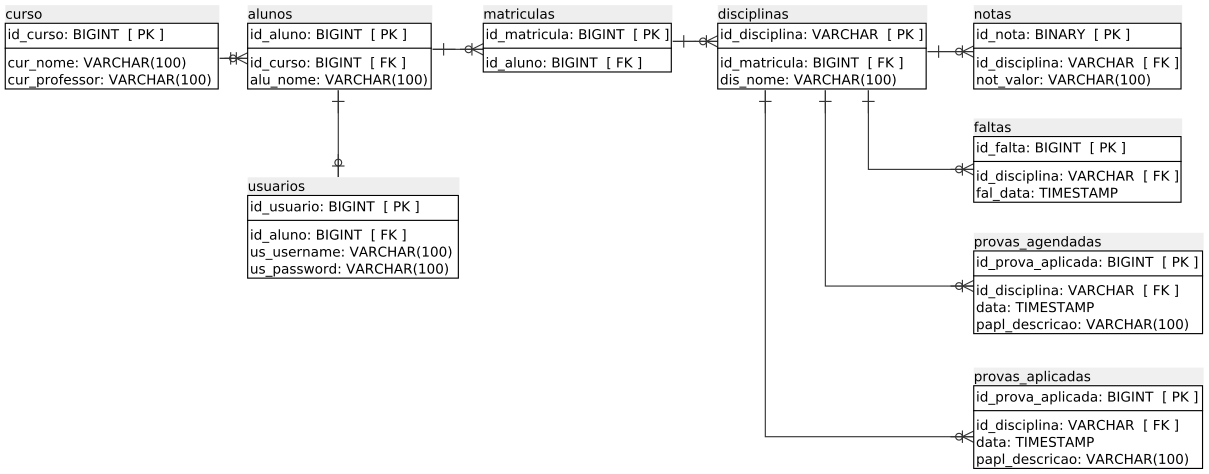
\includegraphics[scale=0.5]{./imagens/imagem5.png}}
			\caption[Diagrama de Entidade e Relacionamento]{Diagrama de Entidade e
			Relacionamento.
			\textbf{Fonte:}Elaborado pelos autores.}
			\label{fig:exemplo5}
		\end{figure}

		\par Fazendo uso desse diagrama foi possível criar todas as classes
	\textit{Java} que representam as entidades do mapeamento objeto-relacional. 
	Essas classes foram criadas fazendo uso de anotações próprias do
	\textit{Hibernate}, que é um \textit{framework} que implementa a especificação
	JPA\footnote{JPA - \textit{Java Persistense API}}. Essas classes fazem parte
	dos mecanismos de persistêcia de dados, e são simplesmente POJO's\footnote{POJO
	- \textit{Plain Old Java Object }} ou seja objetos simples que contêm somente
	atributos privados e os métodos \textit{getters} e \textit{setters} que servem
	apenas para encapsular estes atributos. Uma das classes criadas, foi a classe
	\texttt{Curso.java} que representa a tabela \texttt{cursos} no banco de dados e
	está representada na figura \ref{fig:classecurso}.
	
	\pagebreak
	
	\begin{lstlisting} [style=custom_Java,caption={[Classe \texttt{Curso}]{Classe
	\texttt{Curso}. \textbf{Fonte:} Elaborado pelos autores.}},
	label=fig:classecurso] @Entity(name = "cursos") 
	public class Curso {

			private Long idCurso;
			private String nome;
			private String professor;
		
			@Id
			@GeneratedValue
			@Column(name = "id_curso")
			public Long getIdCurso() {
				return idCurso;
			}
		
			public void setIdCurso(Long idCurso) {
				this.idCurso = idCurso;
			}
		
			@Column(length = 100, nullable = false)
			public String getNome() {
				return nome;
			}
		
			public void setNome(String nome) {
				this.nome = nome;
			}
		
			@Column(length = 100, nullable = false)
			public String getProfessor() {
				return professor;
			}
		
			public void setProfessor(String professor) {
				this.professor = professor;
			}
			
			/**
			 *hashCode e Equals
			 */
		}
	\end{lstlisting}
	
		\par Foram criadas outras classes \textit{Java} com a mesma finalidade da
	anterior, porém com pequenas diferenças no que diz respeito à atributos,
	metodos e anotações. Essas outras classes estão representadas na
	figura \ref{fig:otherclass}.
	
		\begin{figure}[h!]
			\centerline{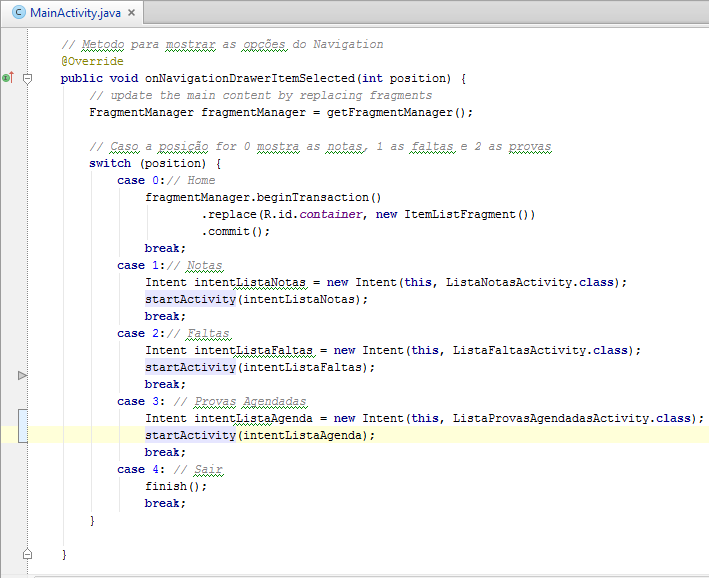
\includegraphics[scale=0.5]{./imagens/imagem6.png}}
			\caption[Classes que Representam Entidades]{Classes que Representam Entidades.
			\textbf{Fonte:}Elaborado pelos autores.}
			\label{fig:otherclass}
		\end{figure}
		
			\par Em seguida à criação das entidades, foi necessário configurar o arquivo
		\texttt{persistence.xml} que fica dentro do \textit{classpath} do projeto
		\textit{Java} ou seja, dentro da mesma pasta onde estão contidas as classes do
		projeto. Esse arquivo é extremamente importante pois, é nele que estão todas
		as configurações relativas à conexão com o banco de dados, configurações
		referentes ao Dialeto SQL que vai ser usado para as consultas e configurações
		referentes ao \textit{persistence unit} que é o responsável direto por
		conversar com obanco de dados. O arquivo \texttt{persistence.xml} está exposto
		na 
	
  \begin{lstlisting} [style=custom_XML]

		<?xml version="1.0" encoding="UTF-8"?>
		<persistence version="2.1"
			xmlns="http://xmlns.jcp.org/xml/ns/persistence" 
			xmlns:xsi="http://www.w3.org/2001/XMLSchema-instance"
			xsi:schemaLocation="http://xmlns.jcp.org/xml/ns/persistence
			http://xmlns.jcp.org/xml/ns/persistence/persistence_2_1.xsd">
				<persistence-unit name="WsUnivas">
					<provider>org.hibernate.ejb.HibernatePersistence</provider>
					<properties>
						<property name="javax.persistence.jdbc.url" value="jdbc:postgresql://localhost:5432/wsunivas" />
						<property name="javax.persistence.jdbc.user" value="postgres" />
						<property name="javax.persistence.jdbc.password" value="2289cpm22" />
						<property name="javax.persistence.jdbc.driver" value="org.postgresql.Driver" />
						<property name="hibernate.dialect" value="org.hibernate.dialect.PostgreSQLDialect" />
						<property name="hibernate.show_sql" value="true" />
						<property name="hibernate.format_sql" value="true" />
						<property name="hibernate.hbm2ddl.auto" value="update" />
					</properties>
				</persistence-unit>
		</persistence>
	\end{lstlisting}
		
		
		\par criação do JpaUtil

		\par criação e disponibilização do primeiro serviço
